\section{Path Planning using Reinforcement Learning}

\subsection{Environment}

The environment used for model training was based on the Fetch Reach environment made available by Gymnasium Robotics (https://robotics.farama.org/envs/fetch/reach/). In this environment, the task was to make the manipulator move the end-effector to a random 3D position above a table in front of the robot, as show in \autoref{fig:fetch_reach_env}. The robot in this simulation has 7-DoF and is controlled by small displacements of the gripper in cartesian coordinates, with Mujoco being responsible for the inverse kinematics computation.

\begin{figure}[H]%[ht]
    \centerline{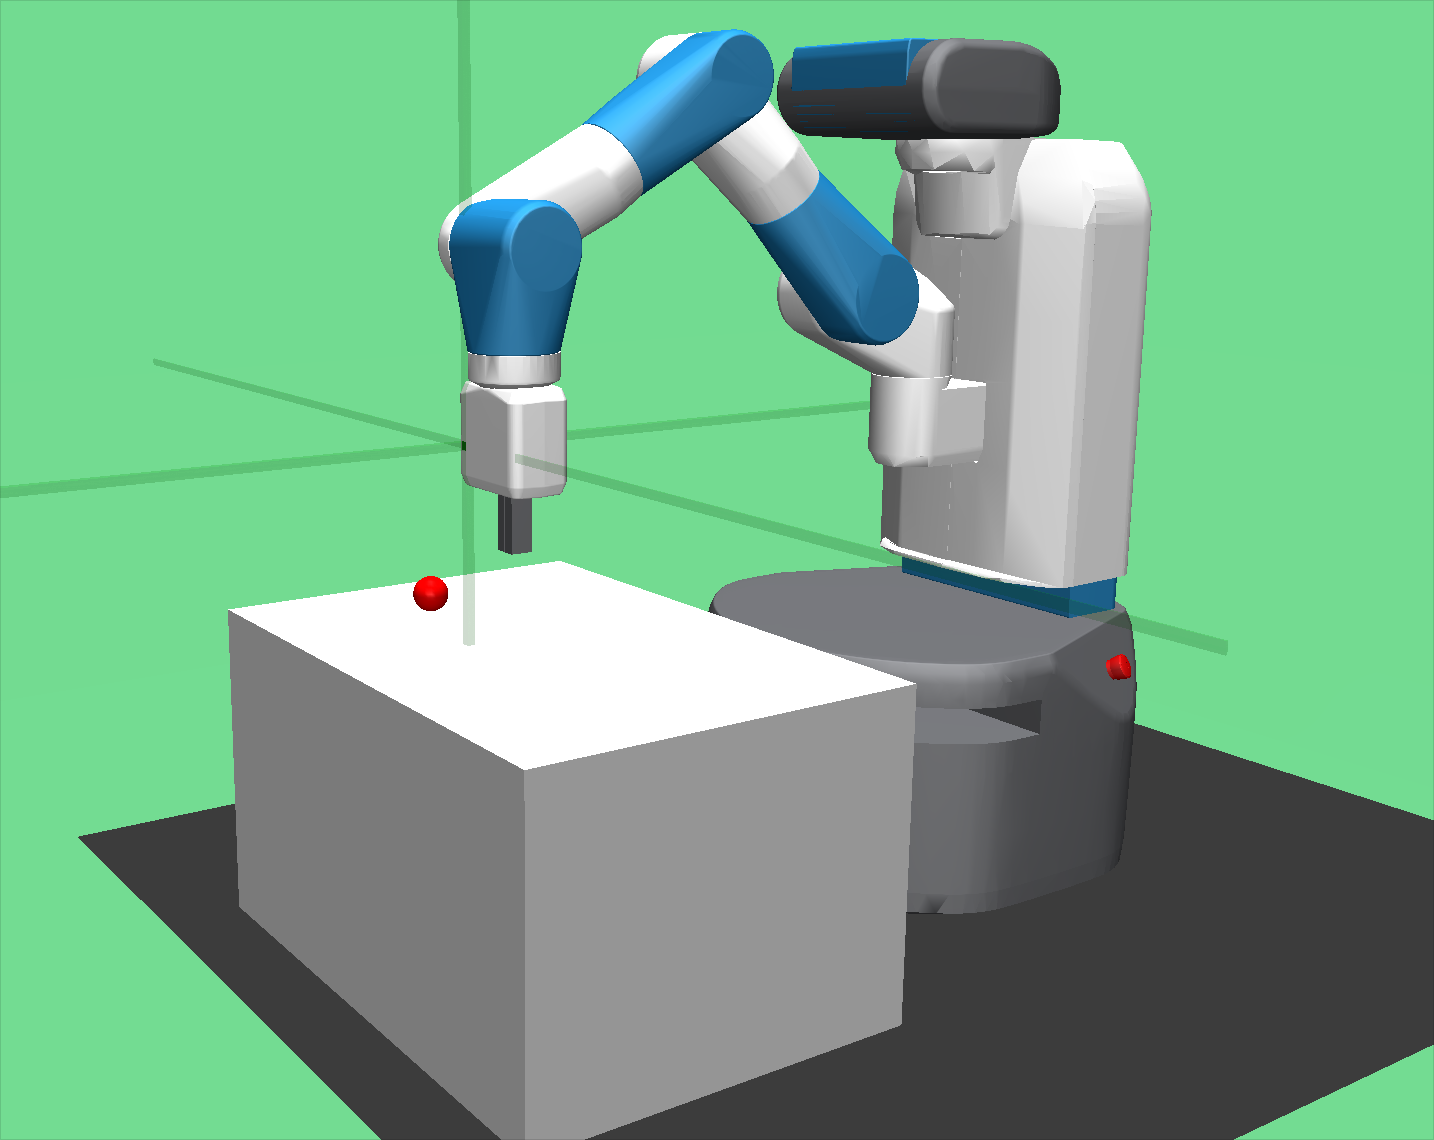
\includegraphics[width=0.7\textwidth]{figs/fetch_reach.png}}
    \caption[Fetch Reach Environment]{Fetch Reach Environment}
    \label{fig:fetch_reach_env}
\end{figure}

The Fetch Reach environment served as a starting point for this research but ended up being mostly rewritten to not only resemble the available collaborative cell but also allow for direct joint control instead of the previous cartesian displacements. The final environment, now named Larcc, can be seen in \autoref{fig:larcc_env} which now includes a UR10e robot model with a Robotiq 2F-140 gripper just like in the real collaborative cell. \textcolor{red}{(should probably refer the sources of the models around here)} The models used were deemed acceptable given that the difference between the end-effector position in ROS and in the simulator differ by less than 1mm for the same joint positions. In this environment, the goal is to move the end-effector to a target position and orientation which are both represented by 3D axes in the simulator. As the actions affect the joints directly, a model trained is this environment ends up replacing the inverse or differential kinematics.

\begin{figure}[H]%[ht]
    \centerline{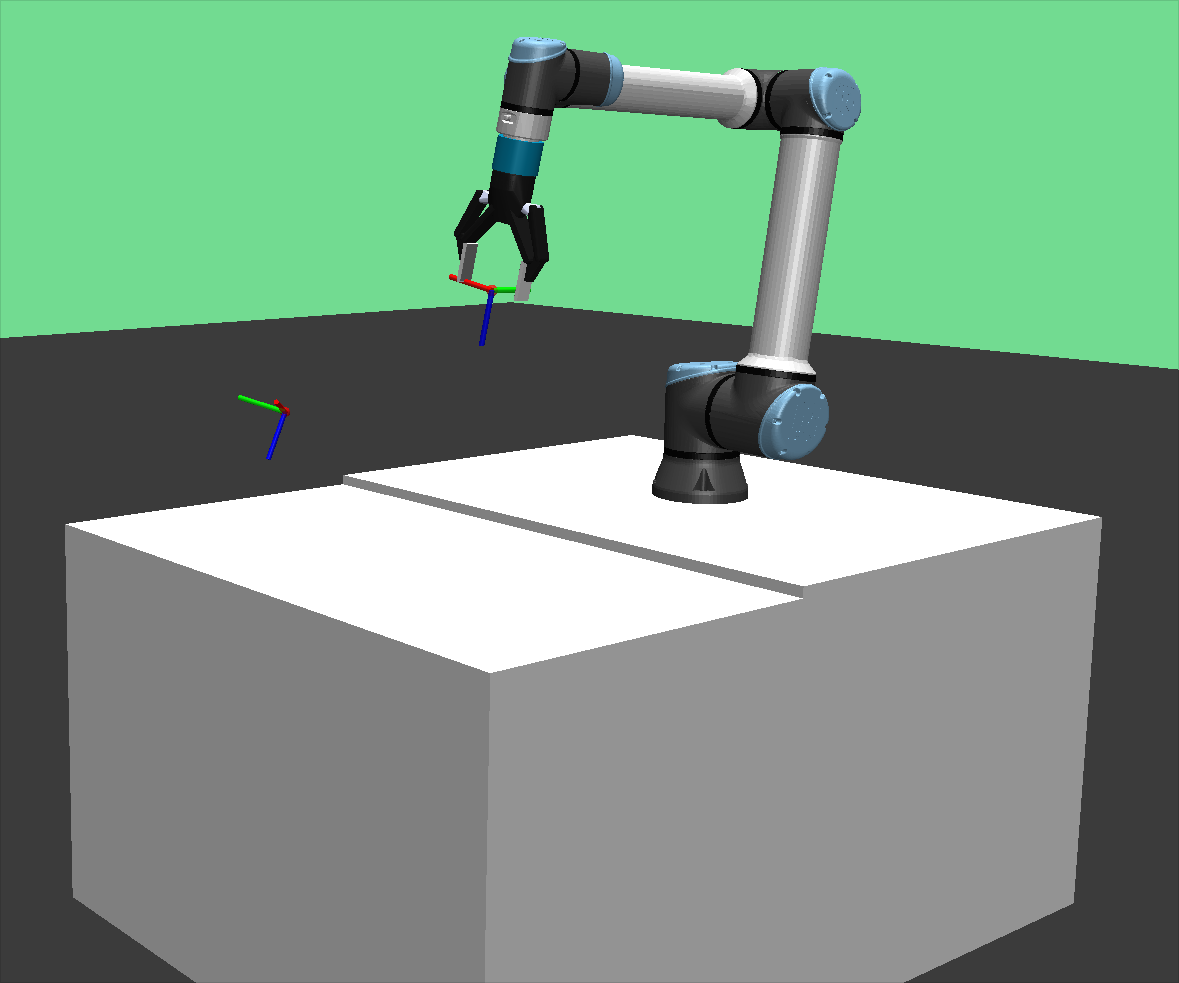
\includegraphics[width=0.7\textwidth]{figs/larcc_env.png}}
    \caption[Larcc Environment]{Larcc Environment}
    \label{fig:larcc_env}
\end{figure}

\subsubsection{Starting State}

\textcolor{red}{currently it is fixed but I hope I can make it random soon!}

\subsubsection{Observation Space}

The observation space in this environment follows the structure commonly used Gymnasium environments being a dictionary with 3 keys:

\begin{itemize}
    \item $observation$: consists of the positions of the 6 joints; given that they were limited to the $[-\pi, \pi]$ interval, they were normalized by a division by $\pi$;
    \item $achieved\_goal$: current position and orientation of the end-effector; the position was normalized by subtracting the position of the robot base link in the environment and then dividing by the arm's range, and the orientation was kept because it is defined with quaternions which are already in the $[-1, 1]$ interval;
    \item $desired\_goal$: position and orientation of the goal; normalized in the same way as the achived\_goal above.
\end{itemize}

\subsubsection{Action Space}

The action space represents the displacements in all joints for a single timestep. These displacements are also normalized which means that the final action applied to the environment is the result of the action output given by a model which is in the $[-1, 1]$ range multiplied by the maximum displacements of the joints. The first two joints associated with the shoulder can move at most 0.8 radians per timestep while the other four joints associated with the elbow and the wrist can move at most 1.2 radians per timestep, representing the different maximum velocities on the UR10e robot joints (https://www.universal-robots.com/products/ur10-robot/).

\subsubsection{Rewards}

\textcolor{red}{(there is probably a better term than dense)}
The used environment has dense rewards, which means that in every timestep the reward will increase if the the end-effector is closer to the goal and decrease otherwise, helping the model learn which actions lead to a successful episode. The reward in each timestep is obtained from the following rewards:

\begin{itemize}
    \item $position$: $1-distance(goal\_pos, end$-$effector\_pos)$ if distance lower than 2 otherwise $-1$ so that it is normalized;
    \item $orientation$: $max(innerproduct(goal\_quaternion, end$-$effector\_quaternion), innerproduct(-goal\_quaternion, end$-$effector\_quaternion)$;
    \item $bonus$: $1$ if goal has been reached else $0$.
\end{itemize}

These rewards affect the final timestep reward with different weights, but the sum of the weights is always equal to $1$ keeping the final reward in the $[-1, 1]$ range.

\subsection{Models}

\subsubsection{Deep Q-Learning (DQN)}

\subsubsection{Soft Actor-Critic (SAC)}

\subsection{Results}
